\documentclass{article}
\usepackage[T1]{fontenc}
\usepackage{lmodern}
\usepackage{graphicx}
\usepackage{amsmath,amssymb}
\usepackage[a4paper,margin=2cm]{geometry}
\usepackage[absolute,overlay]{textpos}
\setlength{\TPHorizModule}{1mm}
\setlength{\TPVertModule}{1mm}
\usepackage[indonesian]{babel}
\usepackage{hyperref}
\setlength{\emergencystretch}{2em}
% unit: Halaman 11

\begin{document}

% === Halaman 11 (python/native) ===

Penjelasan Analitik  P + Q = R

11

Persamaan garis g:    y = mx + c

Gradien garis g:

𝑚= 𝑦𝑝−𝑦𝑞

𝑥𝑝−𝑥𝑞

Perpotongan garis g dengan

kurva y2 = x3 + ax + b adalah: 

     (mx + c)2 = x3 + ax + b

Koordinat Titik R: 

     xr = m2 – xp – xq

     yr = m(xp – xr) – yp  

Sumber gambar: Andreas Steffen, Elliptic Curve Cryptography

% deskripsi: gambar native xref 61
\noindent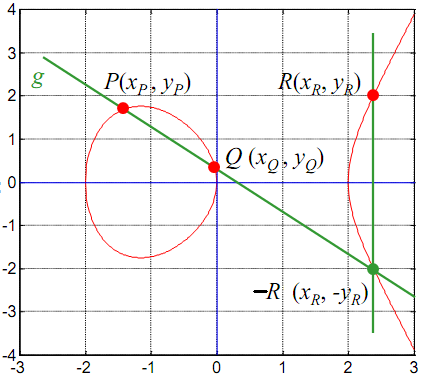
\includegraphics[width=0.85\textwidth]{../../images/python/page_011_img_01.png}

\end{document}
